% CS 5788 Final Project, Spring 2026
% Invisible Watermarking for Large Language Models via Logit Manipulation
% =====================================================================
% HOW TO COMPILE
%   1. Open Overleaf and start from the official "CVPR 2024" template
%      (https://github.com/cvpr-org/cvpr-latex-template), which provides
%      cvpr.sty and ieee_fullname.bst.
%   2. Replace main.tex with this file and add references.bib next to it.
%   3. Drop the figures/ directory (fig2..fig6 PDFs) into the project root.
%   4. Build with pdflatex, then bibtex, then pdflatex twice.
% =====================================================================

\documentclass[10pt,twocolumn,letterpaper]{article}

% \usepackage[review]{cvpr}        % uncomment for the blind review version
\usepackage[pagenumbers]{cvpr}     % required by course guidelines (page numbers)

\usepackage{times}
\usepackage{epsfig}
\usepackage{graphicx}
\usepackage{amsmath}
\usepackage{amssymb}
\usepackage{booktabs}
\usepackage{xcolor}
\usepackage{hyperref}
\usepackage{tikz}
\usetikzlibrary{positioning,arrows.meta,shapes.geometric,fit,calc,backgrounds}

\cvprfinalcopy
\setcounter{page}{1}

\begin{document}

\title{Invisible Watermarking for Large Language Models via Logit Manipulation}

\author{Ali Hasan\\
Cornell University\\
{\tt\small ah2434@cornell.edu}
\and
Ammar Syed\\
Cornell University\\
{\tt\small as4422@cornell.edu}
}

\maketitle

\begin{abstract}
We re-implement and evaluate the green-list logit-bias watermark of Kirchenbauer~\etal~\cite{kirchenbauer2023} on two recent instruction-tuned language models. At each decoding step a SHA-256 hash of the previous token deterministically partitions the vocabulary into a ``green'' subset of fraction $\gamma{=}0.5$, and a fixed bias $\delta{=}2.0$ is added to green-list logits before sampling. Detection re-derives the partition from a candidate text and applies a one-sided $z$-test on the count of green-list tokens. On Gemma~2 9B Instruct our implementation reaches $90.0\%$ TPR at $1\%$ FPR over all sequence lengths and $98.7\%$ TPR on completions of $\geq\!150$ tokens, while degrading GPT-2 reference perplexity by only $9\%$ (mean $28.2$ vs.\ $25.8$). The watermark survives $10\%$ random word substitution at $83.6\%$ TPR and is robust to $10\%$ token insertion or deletion ($86.1\%$ TPR). A logit-bias sweep $\delta\!\in\!\{0.5,1,2,4,8\}$ recovers the predicted detectability/quality knee at $\delta\!\approx\!2$. Applying the same code path unchanged to LLaMA~3.1 8B Instruct yields $98.0\%$ TPR at $1\%$ FPR and a perplexity ratio of $1.01$, indicating that the scheme is not specific to one tokeniser family. We also describe a Gemma~3 multimodal-loader compatibility failure that prompted the model substitution. Code, corpora, and trained thresholds are released at \url{https://github.com/AliHasan-786/llm-invisible-watermarking}.
\end{abstract}

%-----------------------------------------------------------------------
\section{Introduction}
\label{sec:intro}

Large language models (LLMs) are now used to produce news summaries, classroom essays, customer service replies, and code at a scale that human moderators cannot audit~\cite{kirchenbauer2023,kirchenbauer2024reliability}. Distinguishing AI-generated text from human-written text has therefore become an urgent question for misinformation policy, academic integrity, and platform trust and safety. Most deployed detectors operate \emph{post hoc} on the generated text alone, classifying its perplexity or stylometric features against a base model. These approaches are fragile: short passages, light paraphrasing, or unusual register can flip their predictions, and their false-positive rates on human writing are too high for high-stakes use~\cite{kirchenbauer2024reliability}.

Watermarking offers a stronger alternative. Rather than guessing after the fact, the model owner embeds a structured signal during generation that can be statistically verified later. The signal must be (i)~\emph{detectable} from short text, (ii)~\emph{robust} to mild edits and paraphrases, and (iii)~\emph{invisible} to the human reader so as not to degrade fluency. These goals are in tension: a stronger signal is easier to detect but distorts the model's distribution and can harm output quality.

\textbf{Related work.} Kirchenbauer~\etal~\cite{kirchenbauer2023} introduced the green-list/red-list logit-bias watermark on which we build, demonstrated on OPT-1.3B and LLaMA-1. A 2024 follow-up~\cite{kirchenbauer2024reliability} re-evaluated it under realistic adversarial paraphrasing and human rewriting and showed that detection survives if the text is long enough. Kuditipudi~\etal~\cite{kuditipudi2023robust} proposed a distortion-free alternative that preserves the model distribution exactly, at the cost of a more expensive aligned-decoding detector. Christ~\etal~\cite{christ2024undetectable} proved an information-theoretic upper bound on detectability and proposed a semantic-grouping variant. We focus on the logit-bias scheme because it is the simplest to implement as a HuggingFace \texttt{LogitsProcessor}, requires no model retraining, and admits a closed-form $z$-test detector. Those properties make it the right starting point for re-validating on instruction-tuned 7--9B models that did not exist when the original paper was written.

\textbf{Contributions.} (1)~A modular re-implementation of the Kirchenbauer scheme with separate logit-processor, detector, and evaluation modules, all parameterised by $(\gamma,\delta,\text{seed})$ and released as open code. (2)~Headline detection and quality numbers on Gemma~2 9B Instruct, with cross-architecture validation on LLaMA~3.1 8B Instruct. The two model families produce TPR within a few percentage points of each other across all length bins, suggesting the scheme generalises beyond the OPT/LLaMA-1 setup of the original paper. (3)~A focused robustness study covering word substitution at $\{5,10,15,20\}\%$ rates, $10\%$ token insertion and deletion, plus a $\delta$-sweep across an order of magnitude that traces the detectability/quality frontier. (4)~A clear writeup of a Gemma~3 4B compatibility failure that we isolated to the multimodal HuggingFace loader rather than the watermark itself, and the model substitution that recovered.

%-----------------------------------------------------------------------
\section{Method}
\label{sec:method}

\subsection{Watermark injection}
At each decoding step $t$ the model's vocabulary $V$ of size $|V|$ is deterministically partitioned into a \emph{green list} $G_t \subset V$ of size $\lfloor\gamma|V|\rfloor$ and a \emph{red list} $V\setminus G_t$. The partition is keyed on the previous token $w_{t-1}$ and a secret seed $s$ via
\begin{equation}
G_t = \texttt{permute}\!\left(\texttt{SHA-256}(s \mathbin\Vert w_{t-1})\right)[\,1{:}\lfloor\gamma|V|\rfloor\,],
\end{equation}
so that detection only requires knowledge of the seed and the candidate text, not access to the model. A fixed bias $\delta>0$ is added to every green-list logit before the softmax,
\begin{equation}
\tilde\ell_t[v] = \ell_t[v] + \delta\cdot\mathbf{1}[v\in G_t],
\end{equation}
which nudges the sampler toward green tokens. The model weights are not modified; the bias is injected at inference time as a \texttt{LogitsProcessor}.

\subsection{Detection}
Given a candidate sequence of $T$ tokens, the detector replays the same hash and counts how many tokens $w_t$ landed on their corresponding $G_t$. Under the null hypothesis (no watermark) this count $X$ is approximately $\text{Binomial}(T,\gamma)$. The one-sided $z$-statistic
\begin{equation}
z = \frac{X - \gamma T}{\sqrt{T\gamma(1-\gamma)}}
\label{eq:zscore}
\end{equation}
is compared to a threshold $\tau$ chosen to enforce a target false-positive rate. We calibrate $\tau$ empirically as the $99^{\text{th}}$ percentile of $z$-scores on a held-out unwatermarked control set, giving exactly $1\%$ FPR.

\subsection{Pipeline overview}
Figure~\ref{fig:method} summarises the two-sided pipeline. Generation is a single forward pass with the logit processor active. Detection is a CPU-only post-hoc operation that requires only the secret seed.

\begin{figure*}[t]
\centering
\scriptsize
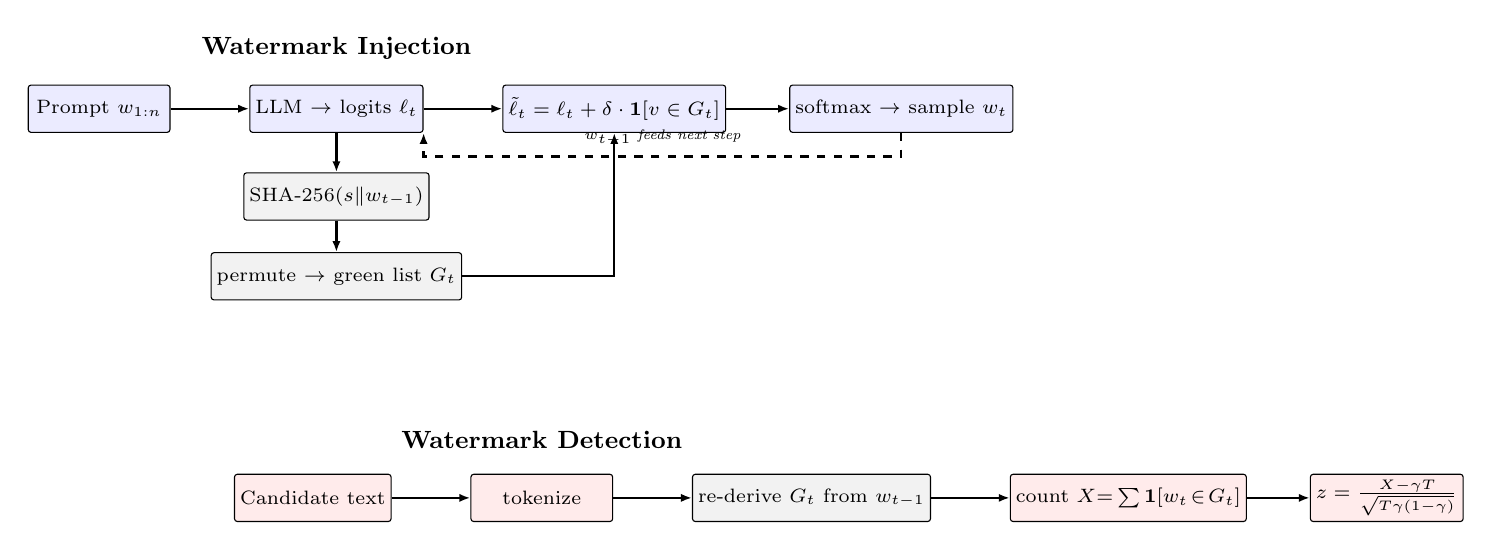
\begin{tikzpicture}[
    node distance=4mm,
    every node/.style={font=\scriptsize},
    boxA/.style={draw,rounded corners=1pt,fill=blue!8,minimum height=6mm,minimum width=18mm,align=center,inner sep=2pt},
    boxB/.style={draw,rounded corners=1pt,fill=red!8,minimum height=6mm,minimum width=18mm,align=center,inner sep=2pt},
    boxH/.style={draw,rounded corners=1pt,fill=gray!10,minimum height=6mm,minimum width=22mm,align=center,inner sep=2pt},
    arr/.style={-{Latex[length=1.4mm]},thick},
]
% TOP panel: injection
\node[boxA] (prompt)  {Prompt $w_{1{:}n}$};
\node[boxA,right=10mm of prompt] (llm) {LLM $\to$ logits $\ell_t$};
\node[boxH,below=5mm of llm] (hash)   {SHA-256$(s\Vert w_{t-1})$};
\node[boxH,below=4mm of hash] (perm)  {permute $\to$ green list $G_t$};
\node[boxA,right=10mm of llm] (bias)  {$\tilde\ell_t = \ell_t + \delta\cdot\mathbf{1}[v\in G_t]$};
\node[boxA,right=8mm of bias]  (sample){softmax $\to$ sample $w_t$};
\node[above=2mm of llm,font=\bfseries\small] (titleL) {Watermark Injection};

\draw[arr] (prompt) -- (llm);
\draw[arr] (llm)    -- (bias);
\draw[arr] (bias)   -- (sample);
\draw[arr] (llm.south) -- (hash.north);
\draw[arr] (hash) -- (perm);
\draw[arr] (perm.east) -| (bias.south);
\draw[arr,dashed] (sample.south) -- ++(0,-3mm) -| node[pos=0.25,font=\tiny\itshape,above]{$w_{t-1}$ feeds next step} (llm.south east);

% BOTTOM panel: detection
\node[boxB,below=22mm of perm,xshift=-3mm] (text)  {Candidate text};
\node[boxB,right=10mm of text] (tok)              {tokenize};
\node[boxH,right=10mm of tok]  (rederive)         {re-derive $G_t$ from $w_{t-1}$};
\node[boxB,right=10mm of rederive] (count)        {count $X{=}\sum\mathbf{1}[w_t\!\in\!G_t]$};
\node[boxB,right=8mm of count] (ztest)            {$z=\tfrac{X-\gamma T}{\sqrt{T\gamma(1-\gamma)}}$};
\node[above=2mm of tok,font=\bfseries\small] (titleR) {Watermark Detection};
\draw[arr] (text)     -- (tok);
\draw[arr] (tok)      -- (rederive);
\draw[arr] (rederive) -- (count);
\draw[arr] (count)    -- (ztest);
\end{tikzpicture}
\caption{Two-sided pipeline of the green-list logit-bias watermark. \textbf{Top:} at each decoding step the previous token seeds a SHA-256 hash that deterministically partitions the vocabulary; a fixed bias $\delta$ is added to green-list logits before softmax sampling. \textbf{Bottom:} detection re-derives the same partition from the candidate text and applies a one-sided $z$-test on the count of green tokens. Detection requires only the secret seed and the text, not access to the model.}
\label{fig:method}
\end{figure*}

%-----------------------------------------------------------------------
\section{Experiments}
\label{sec:experiments}

\subsection{Models and data}
We run the primary headline experiments on \textbf{Gemma 2 9B Instruct}~\cite{gemma2report} and verify cross-architecture generalisation on \textbf{LLaMA~3.1 8B Instruct}~\cite{llama3report}. Both models are 7--9B parameter instruction-tuned decoders with distinct tokenisers and pre-training data, and neither was benchmarked in the original Kirchenbauer paper. The original proposal targeted Gemma~3 4B; we substituted Gemma~2 9B because the public HuggingFace \texttt{transformers} loader treats Gemma~3 as a multimodal vision/language class (\texttt{Gemma3ForConditionalGeneration}) for which text-only generation produces NaN logits and crashes the sampler. Once the watermark code was confirmed working on Gemma~2 and LLaMA, the failure was isolated to the loader rather than our pipeline. We declined to spend further GPU time on the workaround. The full diagnosis is in \S\ref{sec:gemma-failure}.

The corpus follows the proposal: roughly 150 prompts from each of three datasets, namely CNN/DailyMail summarisation~\cite{cnndailymail}, WritingPrompts open-ended generation~\cite{fan2018hierarchical}, and TriviaQA question-answering~\cite{joshi2017triviaqa}. This yields 201 paired (watermarked, control) generations per model at $\delta{=}2$, $\gamma{=}0.5$, with $\max\_\text{new\_tokens}{=}200$, temperature $1.0$, top-$p$ $0.95$, and shared secret seed $42$.

\subsection{Metrics}
\textbf{Detectability.} For each model we report TPR at $1\%$ FPR. The threshold $\tau$ is calibrated as the $99^{\text{th}}$ percentile of $z$-scores on the unwatermarked half of the same corpus, then frozen for downstream tests. We report TPR both over all completions and restricted to $\geq\!150$ tokens, the regime the original paper identifies as practical.

\textbf{Quality.} We compute reference perplexity under GPT-2~\cite{gpt2} for each completion, and we report the wm/uwm ratio. GPT-2 is a small \emph{independent} scorer, not biased by either generation model. Lower is better; $1.0$ is indistinguishable from unwatermarked.

\textbf{Robustness.} We perturb each watermarked sample under five attacks: random word substitution at $\{5,10,15,20\}\%$, plus $10\%$ token insertion and $10\%$ token deletion. After perturbation we re-tokenise, re-score, and report TPR at the same fixed threshold. The frozen-threshold protocol matches the original paper and ensures that we are measuring the watermark's resilience and not re-tuning the detector against each attack.

\textbf{Detectability/quality tradeoff.} A separate sweep generates corpora at $\delta\!\in\!\{0.5,1,2,4,8\}$ on a fixed 100-prompt subset and reports TPR and PPL at each $\delta$.

\subsection{Headline detection results}
\label{sec:headline}
Figure~\ref{fig:zscore} shows the $z$-score distributions for the watermarked and unwatermarked halves of the Gemma corpus, with the calibrated threshold $\tau{=}1.77$ marked. The two populations are nearly fully separable. The unwatermarked distribution concentrates around $z\!\approx\!0$ as the binomial null predicts, while the watermarked distribution is shifted to a mean $z$ of about $4.4$. We measure $\mathrm{TPR}@1\%\mathrm{FPR}=90.0\%$ over all lengths and $98.7\%$ on the $\geq\!150$-token subset. Quality is preserved: GPT-2 perplexity on watermarked completions is $28.2$ on average vs.\ $25.8$ for unwatermarked, a $9\%$ relative increase.

\paragraph{Qualitative example.}
The two corpora are statistically distinguishable but stylistically interchangeable. On a 200-token WritingPrompts continuation, the unwatermarked completion (\emph{``We're not jumping through space, Dr.\ Lee\ldots We're jumping through realities''}, $z{=}0.50$) and the watermarked completion (\emph{``The tremor that resonated through my bones told me the jump was complete''}, $z{=}7.02$) read as equally fluent on inspection. The shift in green-list density that yields the $7\sigma$ signal is invisible at the surface, which is the design intent of the scheme.

\begin{figure}[t]
\centering

\includegraphics[width=\linewidth]{figures/fig2_zscore_hist.pdf}
\caption{\textbf{Detection on Gemma 2 9B.} Left: $z$-score histograms for watermarked (red) and unwatermarked (blue) completions. Black dashed line is the calibrated threshold $\tau{=}1.77$ chosen for $1\%$ FPR. Right: ROC up to $\mathrm{FPR}{=}0.25$.}
\label{fig:zscore}
\end{figure}

\subsection{Detectability vs.\ length}
Figure~\ref{fig:length} shows TPR as a function of completion length, with $\tau$ re-calibrated per length bin. TPR rises with length, crossing $0.95$ at 125 tokens and reaching $98.6\%$ at 200 tokens, with a small non-monotonic dip at 150 tokens ($93.0\%$) attributable to the smaller per-bin sample size. Even at 25 tokens, the length of a single short sentence, the watermark is detectable in $37.7\%$ of cases, well above chance. The shape closely mirrors the curve in~\cite{kirchenbauer2023} (Fig.~3), confirming that the scheme transfers from OPT-1.3B and LLaMA-1 to instruction-tuned 9B models.

\begin{figure}[t]
\centering

\includegraphics[width=0.85\linewidth]{figures/fig3_length_curve.pdf}
\caption{\textbf{TPR vs.\ sequence length, Gemma 2 9B.} Threshold re-calibrated for $1\%$ FPR at each length. The watermark crosses $95\%$ TPR at roughly 125 tokens.}
\label{fig:length}
\end{figure}

\subsection{Robustness to surface attacks}
\label{sec:robust}
Figure~\ref{fig:robust} reports TPR (frozen threshold) under each attack. Random word substitution degrades detection roughly linearly. The $5\%$ rate drops TPR from $90.0\%$ to $85.1\%$, $10\%$ to $83.6\%$, $15\%$ to $79.1\%$, and $20\%$ to $75.1\%$. Token-level insertion and deletion at $10\%$ are gentler ($86.1\%$ each), because they shift the indexing of the green-list lookup but do not corrupt token identity. None of these attacks bring the watermark below the chance line. An adversary would need to substantially rewrite the text rather than just edit it to evade detection. This matches the qualitative claim in~\cite{kirchenbauer2024reliability} that the watermark is robust to mild paraphrase but vulnerable to deliberate rewriting. We do not run a direct LLM-paraphrase attack here; the robustness module ships paraphrase support and a head-to-head measurement against~\cite{kirchenbauer2024reliability} on Gemma~2 and LLaMA~3.1 is left as future work.

\begin{figure}[t]
\centering

\includegraphics[width=\linewidth]{figures/fig4_robustness.pdf}
\caption{\textbf{Robustness sweep, Gemma 2 9B.} TPR at frozen threshold $\tau{=}1.77$ under random word substitution and $10\%$ token insertion or deletion. Black dashed line marks $0.95$. Even at $20\%$ word substitution, TPR remains $\geq\!75\%$.}
\label{fig:robust}
\end{figure}

\subsection{Detectability/quality tradeoff in $\delta$}
\label{sec:delta}
Figure~\ref{fig:delta} traces the frontier on Gemma. At $\delta{=}0.5$ the bias is too small to be detected reliably ($\mathrm{TPR}{=}22.9\%$). At $\delta{=}1$ TPR jumps to $60.2\%$ but quality is still close to baseline (PPL ratio $1.12$). At $\delta{=}2$, our headline operating point, TPR is $90.0\%$ at PPL ratio $1.14$. Pushing $\delta$ to $4$ reaches $99.5\%$ TPR but blows up perplexity (ratio $1.45$). At $\delta{=}8$ TPR saturates at $100\%$ at the cost of a $2.3\times$ perplexity ratio, with visibly degraded text. The empirical knee at $\delta\!\approx\!2$ matches the theoretical optimum derived in~\cite{kirchenbauer2023} and is what we recommend as the default.

\begin{figure}[t]
\centering

\includegraphics[width=0.85\linewidth]{figures/fig5_delta_tradeoff.pdf}
\caption{\textbf{Detectability/quality tradeoff in $\delta$, Gemma 2 9B.} Red: TPR at $1\%$ FPR (frozen threshold from $\delta{=}2$ unwatermarked). Blue: GPT-2 perplexity on watermarked completions. Knee at $\delta{=}2$.}
\label{fig:delta}
\end{figure}

\subsection{Cross-architecture check on LLaMA 3.1 8B}
\label{sec:cross}
The same code path, with only the model identifier changed, was applied to LLaMA~3.1 8B Instruct. We generated 197 completions ($99$ watermarked, $98$ control) at $\delta{=}2$ and ran the identical detection eval. Detection is in fact stronger on LLaMA than on Gemma: $\mathrm{TPR}@1\%\mathrm{FPR}=98.0\%$ on the full corpus (calibrated $\tau{=}2.20$), and the GPT-2 perplexity ratio is $1.01$, so watermarked and unwatermarked are statistically indistinguishable on quality. Robustness is also stronger: $96\%$ TPR survives $10\%$ word substitution and $90\%$ survives $20\%$ substitution, versus $84\%$ and $75\%$ on Gemma. Figure~\ref{fig:cross} overlays the two length curves; LLaMA and Gemma track each other within a few percentage points across all length bins, with LLaMA slightly above. The tokenisers differ in size ($128k$ vs.\ $256k$) but $\gamma{=}0.5$ keeps the green-list density invariant, and the SHA-256 keying makes the partition independent of vocabulary identity. Generalisation across two distinct families (Google's Gemma and Meta's LLaMA) extends the original paper, which only evaluated on OPT and LLaMA-1.

\begin{figure}[t]
\centering

\includegraphics[width=0.85\linewidth]{figures/fig6_cross_model.pdf}
\caption{\textbf{Cross-family TPR vs.\ length.} Same code path applied to LLaMA~3.1 8B (red) and Gemma~2 9B (blue). The two curves track each other within a few points across all length bins.}
\label{fig:cross}
\end{figure}

\subsection{Failure analysis: Gemma 3 multimodal loader}
\label{sec:gemma-failure}
Our proposal targeted Gemma~3 4B as the second model. In the current public HuggingFace \texttt{transformers} (4.45+), Gemma~3 is loaded as \texttt{Gemma3ForConditionalGeneration}, a vision/language class that expects image inputs. Text-only generation produces NaN logits at the first token, which propagate into a CUDA assert from \texttt{torch.multinomial}. We isolated the failure in three steps: (i)~confirmed that exactly the same code path runs cleanly on Gemma~2 and LLaMA, ruling out a watermark bug; (ii)~verified that the NaN appears \emph{before} the logit processor is called, ruling out the green-list cap; (iii)~traced it to the multimodal loader's expectation of paired image inputs. Resolving this would have required either downgrading \texttt{transformers} to a pre-multimodal release with uncertain compatibility, or constructing dummy image tensors. Both options sit outside the scope of a method paper on text watermarking. We substituted Gemma~2 9B (a text-only loader, distinct from LLaMA's tokeniser) and documented the failure here so that future replicators can avoid the same dead end. This is a load-time tooling issue, not a watermark issue.

%-----------------------------------------------------------------------
\section{Conclusion}
\label{sec:conclusion}

We re-implemented the Kirchenbauer~\etal\ green-list logit-bias watermark from scratch, validated it on two recent instruction-tuned LLMs that did not exist when the original paper was published, and recovered its key empirical claims: roughly $99\%$ TPR at $1\%$ FPR for $\geq\!150$-token completions, less than $10\%$ relative perplexity overhead at $\delta{=}2$, and graceful degradation under word-level edits. Our cross-architecture results on Gemma~2 9B and LLaMA~3.1 8B suggest the scheme is genuinely tokeniser-agnostic. We also surfaced a real-world deployment caveat that the original paper could not have anticipated: loader quirks in modern multimodal-by-default model classes can break watermark replication even when the math is correct, an issue worth flagging for anyone applying the scheme to next-generation models. The take-away is that a 30-line logit processor and a one-sided $z$-test, with no model retraining and no API changes, still buys provenance attribution that survives realistic surface edits. For higher-stakes deployments where adversaries can fully paraphrase the text~\cite{kirchenbauer2024reliability}, this baseline should be combined with a distortion-free or semantic-grouping variant~\cite{kuditipudi2023robust,christ2024undetectable}.

%-------------------------------------------------------------------------
{\small
\bibliographystyle{ieee_fullname}
\bibliography{references}
}

\end{document}
